\documentclass{article}
\usepackage{amsmath, amssymb, cite, algorithmic, url, braket}
\usepackage{graphicx}
\usepackage{pythonhighlight}
\usepackage[margin=1.5cm]{geometry}
\usepackage[title]{appendix}
\usepackage{listings}
\usepackage{booktabs}

\graphicspath{{../pic/}}
\lstset{
language=[ANSI]{C},
showtabs=true,
tab=,
tabsize=2,
basicstyle=\ttfamily\footnotesize,%\setstretch{.5},
stringstyle=\color{stringcolour},
showstringspaces=false,
alsoletter={1234567890},
otherkeywords={\%, \}, \{, \&, \|},
keywordstyle=\color{keywordcolour}\bfseries,
upquote=true,
morecomment=[s]{/*}{*/},
commentstyle=\color{commentcolour}\slshape,
literate=*%
{=}{{\literatecolour=}}{1}%
{-}{{\literatecolour-}}{1}%
{+}{{\literatecolour+}}{1}%
{*}{{\literatecolour*}}{1}%
{!}{{\literatecolour!}}{1}%
{[}{{\literatecolour[}}{1}%
{]}{{\literatecolour]}}{1}%
{<}{{\literatecolour<}}{1}%
{>}{{\literatecolour>}}{1}%
% {>>>}{\pythonprompt}{3}%
,%
frame=trbl,
rulecolor=\color{black!40},
backgroundcolor=\color{white},
breakindent=.5\textwidth,frame=single,breaklines=true
}

\begin{document}
\title{DSP Homework 05}
\author{Xu, Minhuan}
\maketitle
\tableofcontents
\begin{abstract}
    \subsubsection*{Summary and Thoughts}
    To sum up the videos we watched this week, and to find out why sunshine is good for us.
    \subsubsection*{Improvement of Our Sampling}
    I proved that we can choose square wave as sampling function rather than $\delta(t)$.
    \subsubsection*{Speed Test of Running}
    I will try to do the thought expriment of using electromagnetic wave and ultrasound wave to measure the speed.
    \subsubsection*{Derivation of Fomulas}
    I derived the result of the Shannon/Nyquist sampling theorem and the perfect reconstruction formula.
\end{abstract}

\section{Summary and Thoughts}

\subsection{Mental Health}
This lecture want to tell us what is important to improve our mental health. There are 8 principles the lecturer mentioned.
\subsubsection*{nutrition}
The research shows that those whose norm was to achieve 100 years or older had the basis of their diet plant-based.
\subsubsection*{exercise}
Exercise help our body produce good happy chemicals.

\subsubsection*{water}

70 percent of our body is water. Water helps to travel nutrients to our brain which are the raw materials of the chemicals mentioned above, and then helps you to become happy.

\subsubsection*{sunshine}

The sunshine make our sleep sounder, and decrease the pain someone has.

\subsubsection*{temperance}

Don't use too much cigarettes, alcohol and coffee.

\subsubsection*{air}

Help clarify our blood.

\subsubsection*{rest}

This world is almost outcome driven, we all want to do much better. But, in the process of pushing ourselves ,we often underestimate the effect of rest and overestimate the effect of the time we spent.

\subsubsection*{trust}
The lecturer quote the words from Ellen White:
\begin{quote}
    The greatest want of the world is the want of $\cdots$ men whose conscience is as true to duty as the needle to the pole; men who will stand for the right though the heavens fall.
\end{quote}
Nowadays, many people have lost in the competition with others and  have given up the basic trust between people around them.
What we should treasure is the pure thoughts we had once we were a baby. In this video, such as, love and trust.

\subsection{Our Planet}
This video shows us the beautiful scenes of shallow seas in earth and the danger of the animals and plants in those areas face.

We human's activities have been effecting the balance of the shallow seas which are the habitat of the living things.

One is the emitting of $CO_2$ , which is one of the results of global warming. In this video, the little change will let the coral get white and die.

The other is fishing. Over fishing break the food chain in the ecological system, which will lead to, in this video, sea urchins falling the kelp forests.

Thankfully, we human have taken action to prevent the bad things from happening. The seas around Misool, mentioned in the last part of this video, has been set as a protected area. In a decade, the vivid scene recovered, and this gives us confidence to make other areas vivid again.

\subsection{New Fuel}
First, this video makes a comparison between the hydrogen, the kerosene and methane.

The hydrogen has good performance as fuel. It can give more impulse with less mass. But it is hard to store because the small density of itself.

The kerosene is easier to store than hydrogen, but the problem is that it cannot be fully burn (into carbon dioxide and water). This makes the residue which is solid have the change of getting stuck in the engine.

The methane achieve the balance of the two fuels. But also that means methane doesn't have the best effect in every area.

The goodness of the methane is that it can be synthesized from $CO_2$. Also, the raw material of this chemical reaction which is carbon dioxide is easy to get on Mars. And if we can get $H_2O$ on Mars, this reaction can even provide excess of oxygen for human breathing. This extra bonus helps us make human settlement in the future.

The scientists are now developing a new technology which can better solve the energy problem on Mars. Moreover, carbon capture on Earth is more to look forward to. If we can improve the efficiency of the reaction which change the carbon dioxide to methane, a clean renewable way of consuming the energy can be found.


\subsection{Thoughts}

In the video of mental health, the lecturer telled us that sunshine is good for our health. But he mentioned little about why the sunshine is good for us. So I searched on the Internet and found the points below.

\subsubsection*{Improves your sleep}

Your body creates a hormone called melatonin that is critical to helping you sleep. Sunshine regulates your circadian rhythm by telling your body when to increase and decrease your melatonin levels. So, the more daylight exposure you can get, the better your body will produce melatonin when it’s time to go to sleep.

\subsubsection*{Maintains strong bones}
One of the best (and easiest) ways to get vitamin D is by being outside. Our bodies produce vitamin D when exposed to sunlight—about 15 minutes in the sun a day is adequate if you’re fair skinned. And since Vitamin D helps your body maintain calcium and prevents brittle, thin, or misshapen bones, soaking in sun may be just what the doctor ordered.

\subsubsection*{Fights off depression}
It’s not just in your head; there’s a scientific reason being in the sunshine improves your mood. Sunshine boosts your body’s level of serotonin, which is a chemical that improves your mood and helps you stay calm and focused. Increased exposure to natural light may help ease the symptoms of seasonal affective disorder --- a change in mood that typically occurs in the fall and winter months when there are fewer hours of daylight.


\section{Problem 2}

\subsection{Restatement}
In the development of the Shannon/Nyquist sampling theorem, the impulse function $\delta (t)$ is used. But $\delta (t)$ is not a practical signal. Does that mean that when applying the sampling theorem in practice, we need some approximation/modification? If yes, what is it that needs to be further done? If no, why?

\subsection{Improvement}

Though the $\delta (t)$ function isn't a practical signal, but it works well in our thought expriment. We should try to use some other similar signals to do the sampling, such as the square wave. Square function has finite values, but has infinite derivative values. It is also a function that hard to generate, but it is realizable. To explore whether this method is good, we should try to find out the expression of $\widetilde{x}_s(t)$ first.

If we let the square wave last the length of $2\tau$, we now have
\begin{equation}
    \begin{aligned}
        s(t) & = \sum_{n = -\infty}^{\infty} \mathrm{rect} (\frac{t - nT}{\tau})                                                                                                    \\
             & = \sum_{n = -\infty}^{\infty}F_n e^{j2 \pi n f_s t}                                                                                                                  \\
             & = \sum_{n = -\infty}^{\infty}\left[ \frac{1}{T} \int_{-\frac T2}^{\frac T2} \mathrm{rect}(\frac{t}{\tau}) e^{-j2 \pi n f_s t} \mathrm{d}t \right] e^{j2 \pi n f_s t} \\
             & = \sum_{n = -\infty}^{\infty}\left[ f_s \int_{-\tau}^{\tau} e^{-j2 \pi n f_s t} \mathrm{d}t \right] e^{j2 \pi n f_s t}                                               \\
             & = \sum_{n = -\infty}^{\infty}2f_s\, \mathrm{sinc} \,( 2f_s n\tau)\, e^{j2 \pi n f_s t} \label{rect_st}                                                               \\
    \end{aligned}
\end{equation}

Therefore
\begin{equation}
    \begin{aligned}
        \widetilde{s}(f) & = \sum_{n = -\infty}^{\infty}\, 2f_s \mathrm{sinc}\, ( 2f_s n\tau)\, \delta(f - nf_s) \\
    \end{aligned}
\end{equation}

And considering the expression below
\begin{equation}
    \begin{aligned}
        \widetilde{x}_s(f) & = \frac{1}{f_c} \cdot \widetilde{x}(f) * \widetilde{s}(f)                                                                                  \\
                           & = \frac{1}{f_c} \cdot \widetilde{x}(f) * \sum_{n = -\infty}^{\infty}\, 2f_s \mathrm{sinc}\, ( 2f_s n\tau)\, \delta(f - nf_s)               \\
                           & = \frac{1}{f_c} \cdot \sum_{n = -\infty}^{\infty}\, 2f_s \mathrm{sinc}\, ( 2f_s n\tau)\, \left[ \widetilde{x}(f) *\delta(f - nf_s) \right] \\
                           & = \sum_{n = -\infty}^{\infty}\,\frac{2f_s}{f_c} \mathrm{sinc}\, ( 2f_s n\tau)\, \widetilde{x}(f - nf_s)
    \end{aligned}
\end{equation}

If we find a LPF $H_a(f)$ whose transfer function is $1$ over $[2f_s T \mathrm{sinc}\, ( 2f_s\tau)]$ and bandwidth $f_c$ is between $B$ and $f_s - B$. Then we have
\begin{equation}
    \widetilde{x}_s(f) \cdot H_a(f) = \widetilde{x}(f)
\end{equation}

Now I has proved the perfect square wave can be used in the sampling. If we find a way to make the rise time of a ladder-shaped function far less than the $\tau$, this function can be used as the square wave, which makes this kind of sampling reasonable.


\section{Speed Test of Running}

\subsection{Restatement}
Find a way to measure your maximum \emph{instantaneous} running speed, accurate to 1mm/s (millimeter per second).

\subsection{Requirement Analysis}
\label{prepare}
To achieve the accuracy, I should find a way to estimate the error value which is uncertainty (Modified by myself).

To calculate the uncertainty of a variable like speed which is the quotient of 2 other variables, we need the fomula below,
The $U~$ are the uncertainty of the 3 variables, and $z = \frac{x}{y}$.


\begin{align}
    \frac{U_z}{z} & = \sqrt{ (\frac{\partial z}{\partial x} \frac{U_x}{x})^2 +  (\frac{\partial z}{\partial y} \frac{U_y}{y})^2} \label{fomula} \\
                  & = \sqrt{ ( \frac{U_x}{x})^2 +  (\frac{U_y}{y})^2}
\end{align}

And for example, we have $v = \frac{x}{t}$, I will suppose the uncertainty of the time $t$ and the distance $x$ all be the division value of the measuring instrument (For the rulers we all have, 1mm).



\subsection{Electromagnetic Wave}
The Doppler shift for relatively low velocity sources is given by
\begin{equation}
    \frac{\Delta f}{f} = \frac{v_s}{c}
\end{equation}
Because the wave incident on the moving car is Doppler shifted and an additional shift because the reflection is from a moving object. The frequency shift of the reflected wave received at the source of the wave is
\begin{equation}
    \frac{\Delta f}{f} = \frac{2 \cdot v_{target}}{c}
\end{equation}
If we need a accuracy of $1~\mathrm{mm/s} = 10^{-3}~\mathrm{m/s}$, we can choose a source of $10~\mathrm{GHz}$, so
\begin{equation}
    \begin{aligned}
        \Delta f & = \frac{2f}{c} \cdot v_{target}                        \\
                 & = \frac{2 \times 10^{10}}{3\times10^{8}} \cdot 10^{-3} \\
                 & \approx 0.07
    \end{aligned}
\end{equation}

This equation reflects a linear relation between $\Delta f$ and $v_{target}$.

So, if we have a device that can distinguish $0.05~\mathrm{Hz}$ of the Delta of source and reflected waves' frequency, we could make the error under $1\mathrm{mm/s}$. I have no idea if we can realize such accuracy.

\subsection{Ultrasound}
In this plan, I will keep sending ultrasound wave at intervals of $T$ and record the time $t$ once the wave send and return. If we have 2 neighbouring points of $t$, and I let the difference value of two $t$ be $\Delta t$. Therefore, It's easy to know that
\begin{equation}
    v_{target} = \frac{V_{sound}  \cdot \Delta t}{T - \Delta t}
\end{equation}
\
Put this in Equa.\ref{fomula}, the uncertainty can be calculated as below

\begin{equation}
    \label{uncertainty}
    \frac{U_{v_t}}{v_t} = \sqrt{\frac{V_{sound}T}{(T-\Delta t)^2} \frac{U_{\Delta t}^2}{(\Delta t)^2}}
\end{equation}

Since we need the accuracy of $1~\mathrm{mm/s}$, the left hand side should be $\frac{U_{v_t}}{v_t} = 10^{-4}$. Other parametres should be as below

\begin{equation*}
    \left\{
    \begin{array}{ll}
        T         & \approx 10^{-1} ~ \mathrm{s}     \\
        V_{sound} & \approx 313.6 ~ \mathrm{m/s}     \\
        v_t       & \approx 5 \sim 10 ~ \mathrm{m/s} \\
        \Delta t  & \approx 10^{-3} ~ \mathrm{s}
    \end{array}
    \right.
\end{equation*}

Put these equations in Equa.\ref{uncertainty}, we can get

\begin{gather}
    \frac{U_{\Delta t}}{\Delta t} = 10^{-6}\\
    U_{\Delta t} \approx 10^{-9}
\end{gather}

That means we cannot make mistake in the order of magnitude of $10^{-9}$, which is also hard to realize.


\section{Problem 4}
\subsection{Restatement}
Derive the result of the Shannon/Nyquist sampling theorem and the perfect reconstruction formula which is as below.
\subsubsection*{Nyquist sampling theorem}

if no actual information is lost in the sampling process, there must be
\begin{equation}
    f_s \geq 2B
\end{equation}
in which B is the bandwidth of the original signal.

\subsubsection*{Perfect Reconstruction Formula}
\begin{equation}
    x(t) = 2f_s T \sum_{n = -\infty}^{\infty} x(nT) ~ \mathrm{sinc} \left[ 2f_s (t - nT) \right]
\end{equation}
\subsection{Proof}
\subsubsection*{Nyquist sampling theorem}

When $x(t)$ is a function with the Fourier transform $\widetilde{x}(f)$
we have the sampling functions below:
\begin{align}
    s(t) & =
    \left\{
    \begin{array}{lr}
        \delta(t - nT) & t = nT             \\
        0              & \mathrm{otherwise}
    \end{array}
    \right. \nonumber                                   \\
         & = \sum_{n = -\infty}^{\infty} \delta(t - nT)
\end{align}

Assuming that $\widetilde{x}(f)$ is the , it is easy to write the sampled $x_s(t)$ as:
\begin{align}
    \because x_s(t)               & = x(t)\times s(t) \nonumber                                    \\
                                  & = \sum_{n = -\infty}^{\infty} x(nT) \delta(t - nT) \label{xst} \\
    % &= x(t) \times \sum_{-\infty}^{\infty} \delta(t - nT)\\
    % &=  \sum_{-\infty}^{\infty} x(nT)~\delta(t - nT)
    \therefore \widetilde{x}_s(t) & = \widetilde{x}(f) * \widetilde{s}(f) \label{xn}
    % &= X(f) * \mathcal{F}\left[\sum_{n = -\infty}^{\infty} \delta(t - nT)\right]
\end{align}

To calculate $\widetilde{s}(f)$, we should find out the Fourier series of ${s}(t)$ first.

Assuming that
$$
    f_s = \frac{1}{T}
$$
$$
    {s}(t) = \sum_{n = -\infty}^{\infty} F_n e^{j2\pi n f_s ~ t}
$$

Easy to find that

\begin{align*}
    F_n & = \frac{1}{T} \int_{- \frac{1}{T}}^{\frac{1}{T}} \sum_{n = -\infty}^{\infty} \delta(t - nT) e^{-j2\pi n f_s ~ t} ~\mathrm{d}t \\
        & = \frac{1}{T} \int_{- \frac{1}{T}}^{\frac{1}{T}} \delta(t) ~\mathrm{d}t                                                       \\
        & = \frac{1}{T}                                                                                                                 \\
        & = f_s
\end{align*}

Therefore
$$
    {s}(t) = f_s \sum_{n = -\infty}^{\infty}e^{j2\pi n f_s ~ t}
$$

Therefore
\begin{align}
    \widetilde{s}(f) & = f_s \sum_{n = -\infty}^{\infty} \mathcal{F} \left[ e^{j2\pi n f_s ~ t} \right]  \nonumber \\
                     & = f_s \sum_{n = -\infty}^{\infty} \delta(f - nf_s)
    \label{sf}
\end{align}

Put Equa.\ref{sf} with Equa.\ref{xn}, we have

\begin{align}
    \widetilde{x}_s(t) & = f_s \sum_{n = -\infty}^{\infty} \widetilde{x}(f) * \delta(f - nf_s) \nonumber \\
                       & = f_s \sum_{n = -\infty}^{\infty} \widetilde{x}(f - nf_s)
\end{align}

In Fig.  we can see there are lots of shifted $\widetilde{x}(f)$ in the spectrum of $\widetilde{x}_s(t)$. The center frequencies of $\widetilde{x}(f)$ are $f_s$ away from each other, so if we don't want the spectrum of them to mix up, we should make
$$
    f_s \leq 2B
$$

\begin{figure}[htbp]
    \centering
    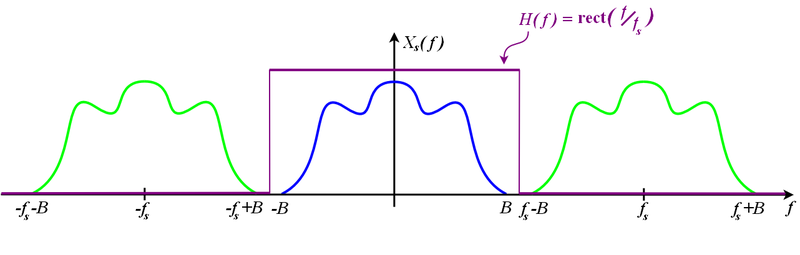
\includegraphics[keepaspectratio,width=250pt]{sampling.png}
    \caption{Spectrum of $\widetilde{x}_s$}\label{sampling}
\end{figure}

\subsubsection*{Perfect Reconstruction Formula}

To prove this equation, we need to calculate $x(t)$
\begin{align}
    x(t) & = \frac{1}{f_s} \mathcal{F}^{-1} \left[ \widetilde{x}(f) \right] \nonumber \\
         & = \frac{1}{f_s} \left[ x_s(t) * h(t) \right] \label{xt}
    % &= \left[ \left( \sum_{n = -\infty}^{\infty} \delta(t - nT) \right) \left( 2fc \mathrm{sinc} 2f_c t \right) \right]
\end{align}
The $h(t)$ is the transfer function of the LPF (like the one in Fig.\ref{sampling}).

\begin{align}
    \because \widetilde{h}(f) & = u(f + f_c) - u(f - f_c)\nonumber                                        \\
    \therefore h(t)           & = \int_{-f_c}^{f_c} e^{j2 \pi ft} ~ \mathrm{d}f \nonumber                 \\
                              & = \left[ \frac{1}{j2 \pi t} e^{j2 \pi t f} \right]_{-f_c }^{f_c}\nonumber \\
                              & = \frac{1}{\pi t} \frac{e^{j2 \pi t f} - e^{- j2 \pi t f}}{2j}\nonumber   \\
                              & = 2f_c \frac{\sin 2\pi f_c t}{2f_c \pi t} \nonumber                       \\
                              & = 2f_c \mathrm{sinc} 2f_c t \label{hf}
\end{align}

Put Equa.\ref{hf} in Equa.\ref{xt}, and we have Equa.\ref{xst}, therefore

\begin{align}
    x(t) & = \frac{1}{f_s} \left\{ \sum_{n = -\infty}^{\infty} x(nT) \left[ \delta(t - nT) * 2f_c ~ \mathrm{sinc} 2f_c t \right] \right\}\nonumber \\
         & = 2 \frac{f_c}{f_s} \sum_{n = -\infty}^{\infty}  x(\frac{n}{f_s}) ~ \mathrm{sinc}\left[ 2f_c(t - \frac{n}{f_s}) \right]
\end{align}

\section{Conclusion}
    \subsubsection*{Summary and Thoughts}
    Sunshine can help us manage the production of some important chemicals. That's why we need a lot of sunshine.
    \subsubsection*{Improvement of Our Sampling}
    I believe we can do sampling with square function.
    \subsubsection*{Speed Test of Running}
    The thought expriment failed.
    \subsubsection*{Derivation of Fomulas}
    I derived the result of the Shannon/Nyquist sampling theorem and the perfect reconstruction formula.

% \bibliographystyle{ieeetr}
% \bibliography{../bib/database}

% \begin{appendices}
%     \section{Code Listing}

% \end{appendices}

\end{document}